\section{Vorgehen bei der Risikoanalyse}

Abbildung~\ref{5analysestufen} zeigt schematisch das Vorgehen bei der Risikoanalyse. Es gilt als erstes die zu schützenden \textit{Werte} zu \textit{identifizieren}. Danach ermittelt man die \textit{Bedrohungen}, welche für die vorher ermittelten Werte bestehen. Anschließend müssen die \textit{Schwachstellen} identifiziert werden, durch welche die Bedrohung wirksam werden kann. Anschließend kann man die \textit{Risiken bewerten} mittels der Formel
\\\\
$ Risiko = Bedrohung * Schwachstelle * Wert $
\\\\
und entsprechende \textit{Prioritäten setzten}, was geschützt werden muss. Ist dies geschehen, kann man entsprechende \textit{Gegenmaßnahmen finden}.

\begin{figure}[h]
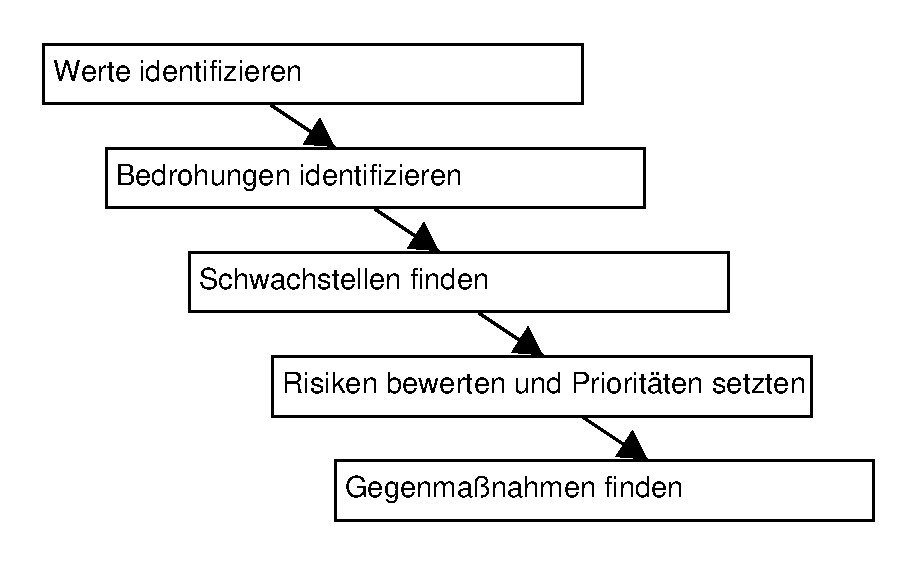
\includegraphics[scale=0.8]{images/5analysestufen.pdf}
\caption{Schematisches Vorgehen bei der Risikoanalyse}
\label{5analysestufen}
\end{figure}



\subsection{Werte identifizieren}
Um die zu schützenden Werte zu identifizieren gibt es mehrere Möglichkeiten. Der einfachste Ansatz ist des, dem Fluss des Geldes zu folgen. \textit{Gegenstände} mit einem festen Preis in der Anschaffung können exakt mit Zahlen erfasst werden. Sie sind relativ leicht für die Wiederbeschaffung im Falle eines Verlustes zu beziffern. Verluste durch den Ausfall von Einkommen lassen sich zwar weniger genau abschätzen, aber sind dennoch gut erfassbar.\\
\textit{Personelle Werte} sind nicht so einfach mit Zahlen zu belegen. Es gibt keine sinnvollen Listenwerte für z.B. den Wert der Kreativität oder Führungskraft einer Person. Scheidet Personal also aus dem Unternehmen aus, aus welchen Gründen auch immer, ist dies schwer zu beziffern.\\
\textit{Daten} jeglicher Art sind weitere wichtige Werte. Der Verlust durch personenbezogene Daten kann mittels Listenwerten aus Studien ermittelt werden, z.B. ~\cite{poneman2014}. Der damit verbundene Imageverlust bei bekanntwerden solcher Vorfälle ist jedoch nicht gut zu ermitteln. Auch Einbußen durch die Preisgabe von Forschungsdaten oder anderen Firmeninterna kann teilweise schwer bewertet werden, da die Art der Weiterverwendung nicht bekannt ist.

\subsection{Bedrohungen identifizieren}
Für jeden Wert, der identifiziert wurde, können Bedrohungen gefunden werden. Einzelne Bedrohungen können mehre Werte bedrohen bzw. sind viele Werte miteinander verbunden. Z.B. bedeutet ein totaler Verlust der Datenbankserver durch eine Flut  zugleich den Verlust der Hardware, wie auch der darauf gespeicherten Daten.

\subsection{Schwachstellen finden}
Damit eine Bedrohung zu einem Risiko werden kann, muss es eine entsprechende Schwachstelle geben, durch die die Bedrohung ausgenutzt werden kann. Im Normalfall gibt es mindestens eine Schwachstelle zu einer Bedrohung, aber z.B. im Falle der Bedrohung durch Hacker über das Internet, gibt es die Schwachstelle einer Verbindung zum Internet nicht, wenn man ein Abgeschlossenes System hat. Bekannte und verbreitete Schwachstellen lassen sich leicht im Netz finden, wie ~\cite{owasp2013} mit den 10 bedeutendsten Schwachstellen und entsprechenden Hinweisen zu Auswirkungen und Schutz.
\subsection{Risiken bewerten und Prioritäten setzten}
Mittels $ Risiko = Bedrohung * Schwachstelle * Wert $ können nun Risiken qualitativ wie auch quantitativ ermittelt werden. Die so ermittelten Risikobewertungen können Prioritäten gesetzt werden, welche Werte besonders geschützt werden müssen und auch wie viele Mittel eingesetzt werden sollten, damit Gegenmaßnahmen sich lohnen. Welche Bereiche genau priorisiert werden, hängt dabei von vielen Faktoren ab, wie der Branche, der Firmenphilosophie, etc..
\subsection{Gegenmaßnahmen finden}
Je nach gesetzten Prioritäten, kann man verschiedene Ansätze verfolgen. Schwachstellen können beseitigt, Bedrohungen verringert werden. Eine andere Möglichkeit ist die Reduzierung der Auswirkungen im Schadensfall. Abbildung~\ref{reduzierungHuefigkeitAusmass} zeigt diese Maßnahmen schematisch.\\
Welcher weg der beste ist, hängt wieder von der Art der Werte ab. Wurden z.B. personenbezogene Daten verloren, ist es für die Betroffenen unwichtig, dass nur ein geringer Prozentsatz der Datensätze offengelegt wurde, der Imageverlust ist trotzdem hoch.\\

\begin{figure}[h]
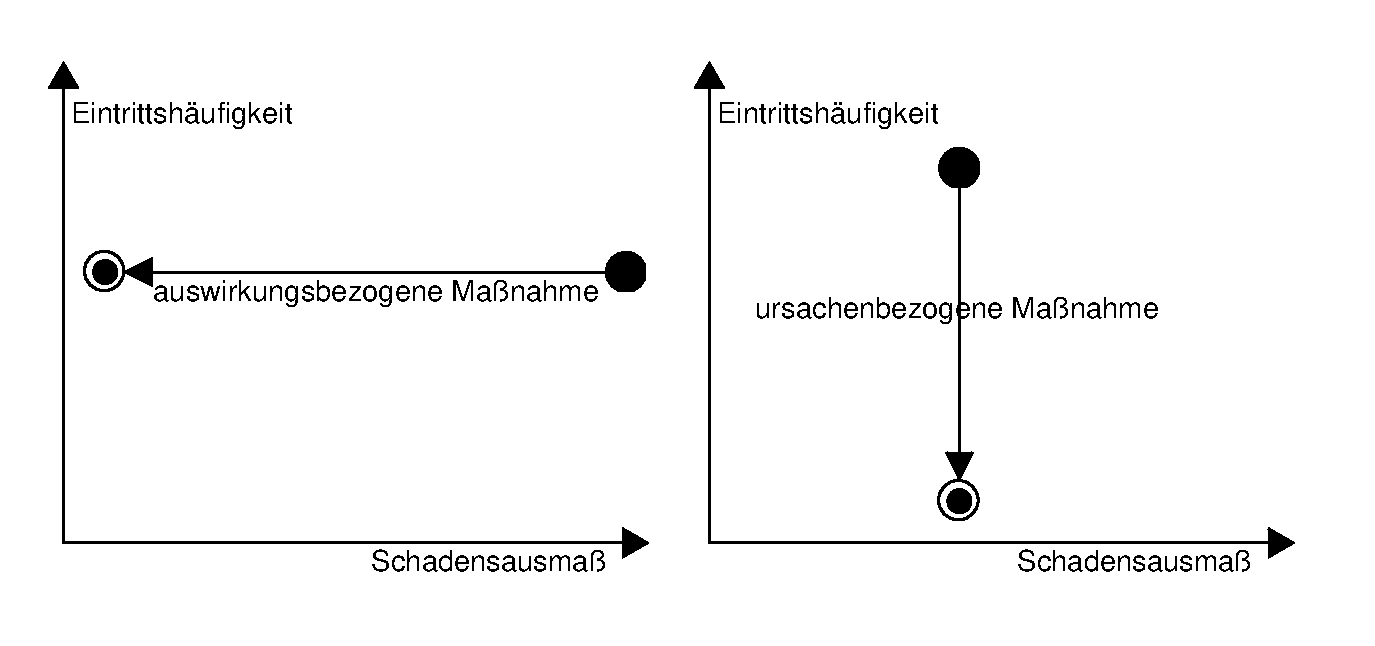
\includegraphics[scale=0.6]{images/reduzierungHuefigkeitAusmass.pdf}
\caption{Schematischer Vergleich von Maßnahmen zur Risikoreduzierung}
\label{reduzierungHuefigkeitAusmass}
\end{figure}

Zu beachten ist, dass das 80-20-Prinzip gilt, man also nie perfekte Sicherheit mit annehmbaren Ausgaben erreichen kann.